\section{Analisis Hasil Pengujian}

\subsection{Siklus Penjualan Tiket}

Kedua skenario pengujian ini memiliki siklus permintaan yang berbeda. Siklus dalam hal ini berarti fase ketika sistem memiliki pola permintaan yang berbeda. Contoh pada skenario beban berkelanjutan diambil dari pengujian f1t2, sedangkan contoh pada skenario perebutan tiket diambil dari pengujian f1t4. Siklus/pola ini juga terjadi pada skenario serupa ketika proses penjualan berjalan dengan lancar.

\subsubsection{Skenario Beban Berkelanjutan}

\begin{figure}[htbp]
    \centering
    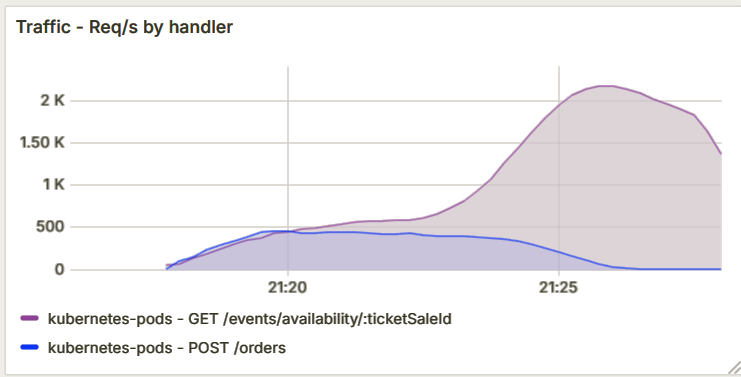
\includegraphics[width=0.6\textwidth]{resources/chapter-4/pattern-stress-traffic.png}
    \caption{Pola Permintaan pada Beban Berkelanjutan}
    \label{fig:pattern-stress-traffic}
\end{figure}

Pada skenario ini, sistem memiliki ketersediaan tiket yang banyak sehingga penjualan tiket yang berhasil berjalan cukup lama. Setelah tiket habis terjual, jumlah permintaan ketersediaan tiket jauh meningkat karena penguji mencoba mencari tiket dari berbagai area dengan lebih banyak.

\begin{figure}[htbp]
    \centering
    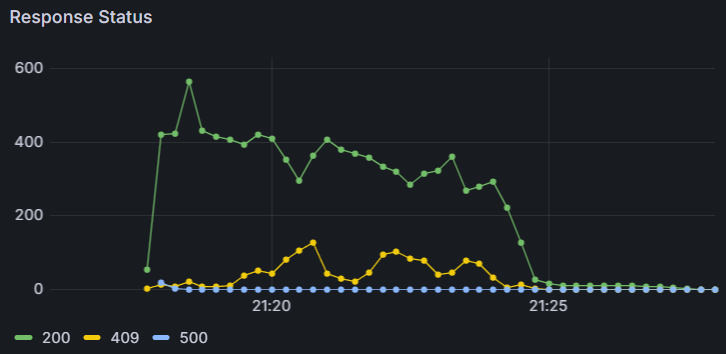
\includegraphics[width=0.6\textwidth]{resources/chapter-4/pattern-stress-order.png}
    \caption{Status Respons pada Beban Berkelanjutan}
    \label{fig:pattern-stress-order}
\end{figure}


Status respons pemesanan tiket menunjukkan bahwa terjadi konflik (kode 409) selama pemrosesan pesanan sebanyak 3-10\% dari respons secara keseluruhan.

\pagebreak

\subsubsection{Skenario Perebutan Tiket}

\begin{figure}[htbp]
    \centering
    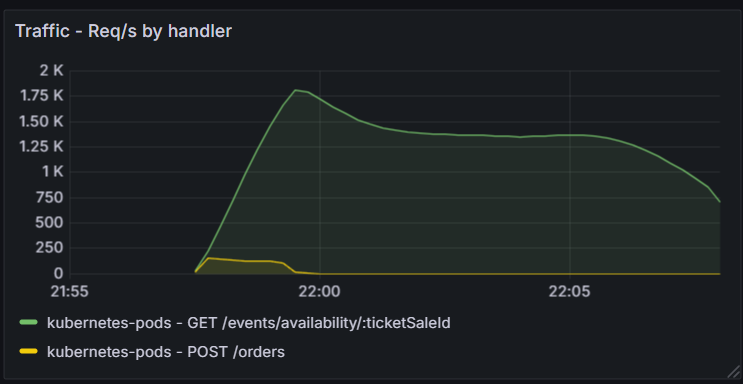
\includegraphics[width=0.6\textwidth]{resources/chapter-4/pattern-sim-traffic.png}
    \caption{Pola Permintaan pada Perebutan Tiket}
    \label{fig:pattern-sim-traffic}
\end{figure}

Pada skenario ini, jumlah permintaan ketersediaan jauh lebih banyak dibandingkan permintaan pemesanan tiket. Hal ini wajar karena terdapat lebih banyak peminat dibandingkan dengan tiket yang tersedia. Berdasarkan grafik di atas, tiket habis terjual dalam kurang lebih 2 menit penjualan.

\begin{figure}[htbp]
    \centering
    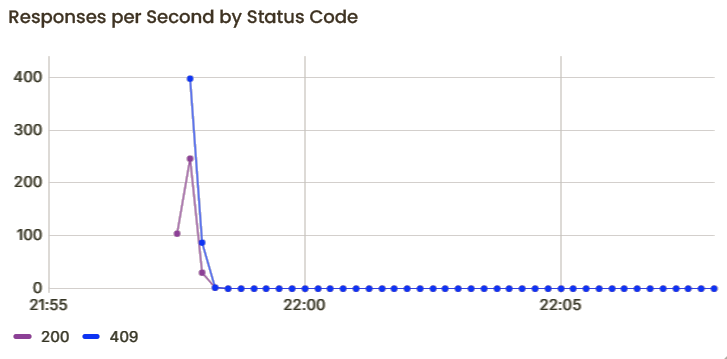
\includegraphics[width=0.6\textwidth]{resources/chapter-4/pattern-sim-order.png}
    \caption{Status Respons pada Perebutan Tiket}
    \label{fig:pattern-sim-order}
\end{figure}

Status respons pemesanan tiket menunjukkan bahwa terjadi konflik (kode 409) yang cukup banyak bahkan sejak proses penjualan dimulai. Pengguna yang baru masuk setelahnya pada akhirnya akan gagal memperoleh tiket, sebagaimana digambarkan pada keadaan akhir penguji pada gambar berikut.

\begin{figure}[htbp]
    \centering
    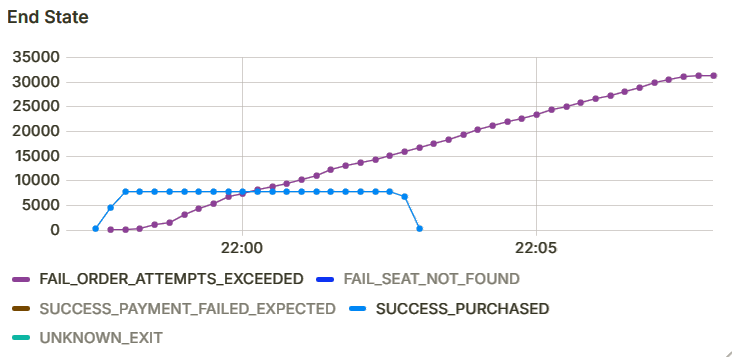
\includegraphics[width=0.6\textwidth]{resources/chapter-4/pattern-sim-k6.png}
    \caption{Keadaan Akhir Penguji pada Perebutan Tiket}
    \label{fig:pattern-sim-k6}
\end{figure}


\subsection{Kinerja Selama Pengujian}

Secara garis besar, varian PostgreSQL mampu menangani beban yang diberikan dengan sangat baik. Varian CitusData masih memiliki kinerja yang baik, meski memiliki latensi yang lebih tinggi dibandingkan dengan PostgreSQL. YugabyteDB mengalami lebih banyak kegagalan dan kinerja yang buruk sehingga tidak dapat menyelesaikan proses penjualan dengan baik. Sampel pengujian yang dipilih pada adalah skenario stress-2 tanpa pengendalian aliran. Skenario ini merupakan skenario pengujian dengan kinerja YugabyteDB yang dapat diterima dan mampu menyelesaikan proses penjualan. Dengan beban yang lebih tinggi, YugabyteDB mengalami banyak kegagalan.

\begin{table}[h]
    \centering
    \caption{Gambaran Kinerja Permosesan Pesanan}
    \label{table:kinerja-pemrosesan-pesanan}
    \begin{tabular}{|l|l|l|l|}
        \hline
        \textbf{Metrik}              & \textbf{PostgreSQL} & \textbf{CitusData} & \textbf{YugabyteDB} \\
        \hline
        \textit{Throughput} Maksimum & 466 rps             & 410 rps            & 216 rps             \\
        \hline
        Penggunaan CPU (Puncak)      & 8 vCPU              & 10 vCPU            & 19 vCPU             \\
        \hline
        Penggunaan Memori (Puncak)   & 3.4 GB              & 5 GB               & 36 GB               \\
        \hline
        Latensi Pemrosesan (P50)     & 192-382 ms          & 496-650 ms         & 854-10000 ms        \\
        \hline
    \end{tabular}
\end{table}

Latensi dan \textit{throughput} pemrosesan diukur dari sisi Ticket Server, bukan dari level basis data. Latensi pemrosesan yang diambil merupakan latensi terbaik saat beban sudah cukup tinggi dan laju pemrosesan mulai stabil. Penggunaan CPU dan penggunaan memori merupakan agregat puncak jumlah penggunaan sumber daya setiap instans basis data yang berkaitan. Apabila terdapat dua nilai maksimal \textit{throughput} yang mendekati, nilai yang dipilih adalah nilai yang memiliki rasio sukses (kode respons 200) paling tinggi.

Berdasarkan tabel di atas, PostgreSQL unggul dari segala aspek, mulai dari laju pemrosesan, penggunaan sumber daya, serta latensi. CitusData memiliki laju pemrosesan yang mendekati PostgreSQL dengan latensi 2x lebih lambat dan penggunaan sumber daya yang sedikit lebih tinggi. Di sisi lain, YugabyteDB memiliki laju pemrosesan kurang dari setengah PostgreSQL dengan latensi setidaknya 4x lebih lambat, penggunaan CPU 2.4x lebih banyak, dan penggunaan memori 10x lebih banyak.

\subsection{Kinerja Basis Data Terdistribusi}

Sebagaimana digambarkan pada tabel \ref{table:kinerja-pemrosesan-pesanan}, kinerja PostgreSQL lebih baik dibandingkan CitusData dan YugabyteDB. Mari telusuri lebih dalam kinerja setiap basis data, terutama pada skenario lain.

\subsubsection{Rata-Rata Waktu Eksekusi Kueri}

Berikut adalah data rata-rata waktu eksekusi kueri yang diambil dari tabel pg\_stat\_statements sesaat setelah pengujian dilaksanakan. Data PostgreSQL diambil dari pengujian f1t2, CitusData diambil dari pengujian f2t3, dan YugabyteDB diambil dari f3t1. Beban antara PostgreSQL dan CitusData sama karena pengujian dijalankan pada skenario stress-0, sedangkan beban pada YugabyteDB lebih ringan karena dijalankan pada skenario stress-2. Data PostgreSQL merupakan gabungan antara statistik pada instans \textit{primary} dan replika. Data mentah merupakan data 10 kueri dengan total eksekusi paling banyak. Kueri yang kosong berarti total eksekusinya tidak cukup signifikan, sehingga dapat diasumsikan latensinya cukup rendah untuk diabaikan dibandingkan dengan yang lain.

\begin{table}[h]
    \centering
    \caption{Latensi Eksekusi Kueri pada Basis Data dalam Milisekon}
    \label{table:latensi-kueri}
    \begin{tabular}{|l|l|l|l|}
        \hline
        \textbf{Kueri}        & \textbf{PostgreSQL} & \textbf{CitusData} & \textbf{YugabyteDB} \\
        \hline
        LockFreeStandingSeats & 8.5                 & 9.8                & 1855                \\
        \hline
        LockNumberedSeats     & -                   & 8.25               & 43                  \\
        \hline
        InsertOrder           & 0.2                 & 4.4                & 77                  \\
        \hline
        UpdateOrder           & -                   & 3.9                & 33                  \\
        \hline
        InsertOrderItem       & 0.24                & -                  & 40                  \\
        \hline
        InsertIssuedTiket     & 0.28                & -                  & 74                  \\
        \hline
        InsertInvoice         & 0.12                & 4.16               & 31                  \\
        \hline
        UpdateInvoice         & 0.12                & 7.7                & -                   \\
        \hline
        UpdateSeatStatus      & 0.06                & 4.34               & 47                  \\
        \hline
        GetAllSeats           & 10                  & 16                 & -                   \\
        \hline
        GetOrderDetail        & 3.5                 & 6.7                & 163                 \\
        \hline
    \end{tabular}
\end{table}

Latensi dan laju pemrosesan yang baik pada PostgreSQL didukung dengan latensi kueri yang rendah. Kueri baca pada CitusData beberapa milisekon lebih lambat dibandingkan dengan PostgreSQL. Perbedaan signifikan terletak pada latensi penulisan yang berada pada ordo milisekon. Bila dibandingkan, latensi penulisan pada CitusData puluhan kali lebih lambat daripada latensi penulisan pada PostgreSQL. Di sisi lain, latensi kueri pada YugabyteDB lebih lambat hingga ratusan kali lipat dibandingkan dengan PostgreSQL baik itu pada kueri baca dan penulisan. Terlebih lagi, YugabyteDB kesulitan menangani kueri LockFreeStandingSeats dengan latensi hingga 1800 milisekon. Perbedaan latensi ini yang membuat laju penulisan CitusData dan YugabyteDB lebih lambat dibandingkan dengan PostgreSQL.

\subsubsection{Pembahasan Kinerja PostgreSQL}

Kinerja PostgreSQL yang baik berasal dari arsitekturnya yang monolitik. PostgreSQL menghindari \textit{overhead} latensi jaringan dan beban koordinasi antar \textit{node}. Beban ini ada pada basis data terdistribusi seperti CitusData dan YugabyteDB. Hal ini terbukti dengan latensi tulis dan baca yang secara konsisten jauh lebih rendah dibandingkan dengan yang lain. Arsitektur inilah yang memungkinkan laju pemrosesan yang tinggi dengan efisiensi penggunaan sumber daya yang baik.

\subsubsection{Pembahasan Kinerja CitusData}

Meskipun secara teori ide pemartisian pada PostgreSQL dengan CitusData terdengar baik, terdapat \textit{tradeoff} dari sisi koordinator yang ternyata tidak dapat diabaikan. Pertukaran ini semakin tidak dapat diabaikan pada kasus penjualan tiket ketika pola kueri adalah banyak kueri ringan yang dijalankan secara berulang-ulang. Perhatikan perbedaan penggunaan sumber daya antara koordinator dan \textit{worker} CitusData pada gambar berikut:

\begin{figure}[htbp]
    \centering
    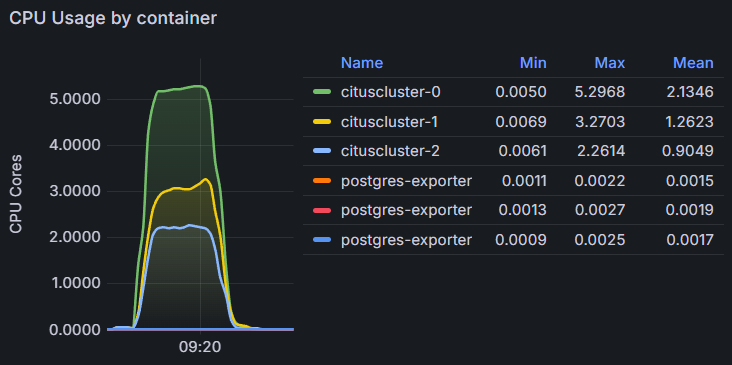
\includegraphics[width=0.8\textwidth]{resources/chapter-4/citusdata-usage.png}
    \caption{Penggunaan CPU CitusData (f2t3)}
    \label{fig:citusdata-usage}
\end{figure}

\textit{Node} cituscluster-0 merupakan koordinator dengan sisanya adalah \textit{worker}. Pada kasus ini, beban pada koordinator cukup tinggi hingga dua kali beban pada satu instans \textit{worker}. Berdasarkan hal tersebut, diketahui bahwa \textit{overhead} pada koordinator memiliki dampak yang signifikan pada kinerja CitusData.

Setelah ditelusuri, terdapat sebuah diskusi pada repositori CitusData yang membahas kinerja CitusData yang buruk pada \textit{benchmark} TPC-C. Terdapat sebuah komentar yang menjawab mengapa hal ini memang wajar. Selain karena CitusData membutuhkan beberapa \textit{network round-trip}, beban TPC-C lebih banyak pada \textit{query planning} dibandingkan dengan eksekusinya \parencite{Slot2020}.

Beban TPC-C dan beban penjualan tiket memiliki kemiripan, sehingga hal yang sama juga berlaku pada kasus ini. Pada penjualan tiket, beban basis data terdiri atas banyak kueri baca dan kueri tulis yang sebenarnya cukup ringan, sehingga koordinator mengalami beban yang tinggi karena harus melakukan tambahan \textit{query planning} untuk koordinasi.

Terdapat alternatif \textit{benchmark} TPC-C yang juga dibahas pada komentar tersebut, yaitu \textit{benchmark} HammerDB. HammerDB menyimpan logika pengujian pada \textit{stored procedure} PostgreSQL. Citus dapat mendelegasikan pemanggilan prosedur tersebut dengan \textit{overhead} yang jauh lebih kecil dan dengan jumlah \textit{network round-trip} yang lebih sedikit \parencite{Slot2020}. Hal ini dibahas lebih lanjut pada artikel yang membahas penggunaan \textit{distributed function} untuk latensi yang lebih baik pada CitusData versi 9 \parencite{Slot2020faster}.

Pendekatan dengan \textit{stored procedure} merupakan alternatif yang dapat dipelajari lebih lanjut pada penelitian lain untuk pengoptimalan yang lebih optimal. Meskipun begitu, permasalahan dari pendekatan ini adalah pemindahan logika bisnis dari kode aplikasi ke basis data. Selain karena keterbatasan sintaks dan dukungan integrasi, logika bisnis yang dijalankan pada level aplikasi belum tentu dapat diterjemahkan secara persis menjadi \textit{stored procedure} PostgreSQL.

\subsubsection{Pembahasan Kinerja YugabyteDB}

Sebagaimana ditunjukkan pada tabel \ref{table:latensi-kueri}, latensi YugabyteDB memang dapat diprediksi karena mekanisme di baliknya yang menggunakan konsensus berbasiskan Raft. Setiap penulisan harus menunggu kluster mencapai konsensus terlebih dahulu, sehingga latensinya lebih tinggi. Meskipun begitu, latensi YugabyteDB yang lebih lambat hingga 100-200x dibandingkan dengan PostgreSQL merupakan hal yang tidak diprediksi.

Pada kasus yang lebih sederhana, seorang pengguna melaporkan penurunan kinerja hingga 300x lebih lambat dibandingkan dengan PostgreSQL. Meski setelah beberapa tahun berlalu telah banyak dilakukan pengoptimalan pada YugabyteDB, referensi hasil pengujian ini tetap dapat dianggap relevan sebagai validasi bahwa penurunan kinerja seperti ini memang juga terjadi pada kasus lain \parencite{yugabyteIssuePerformance}.

Permasalahan latensi ini dapat diterima apabila kinerja YugabyteDB juga diiringi dengan keunggulan dari aspek lain, seperti kemampuan menangani keadaan perebutan tiket dengan baik dan kestabilan kluster yang baik. Meskipun begitu, hal ini juga tidak dapat ditunjukkan oleh YugabyteDB. Berikut adalah gambaran kinerja YugabyteDB saat berjalan dengan baik:

\begin{figure}[htbp]
    \centering
    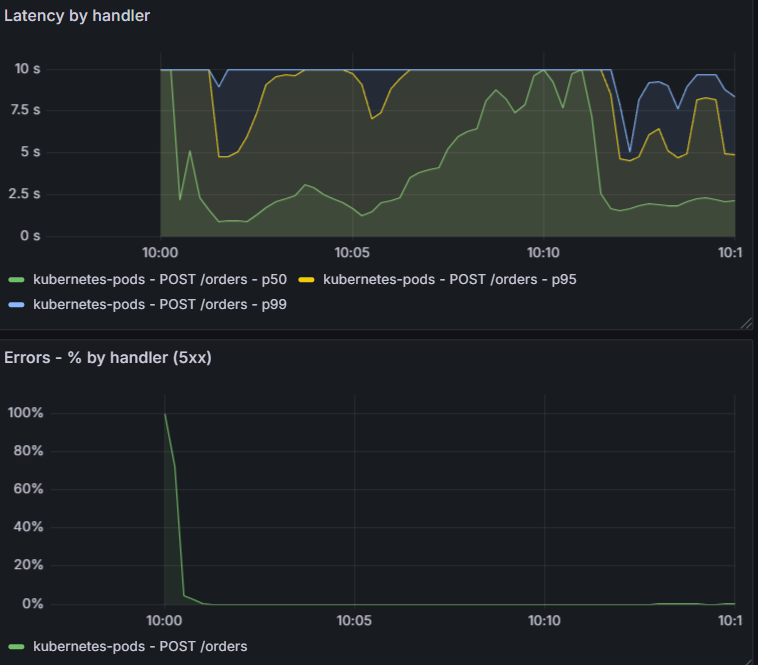
\includegraphics[width=0.8\textwidth]{resources/chapter-4/latensi-yugabyte-success.png}
    \caption{Metrik Pemrosesan Pesanan (f3t2)}
    \label{fig:metrics-f3t1}
\end{figure}

Latensi pemrosesan pada YugabyteDB diawali dengan tingkat kegagalan yang tinggi, lalu pemrosesannya mulai stabil. Setelah itu, latensi pemrosesan mulai meningkat hingga tiba-tiba turun lagi. Hasil ini merupakan hasil paling baik yang dapat diperoleh dari pengujian YugabyteDB. \textit{Tuning} lebih lanjut seperti mengubah batas koneksi dan penambahan beban membuat YugabyteDB mengalami kegagalan penuh sebagaimana terjadi pada hasil pengujian lain:

\pagebreak

\begin{figure}[htbp]
    \centering
    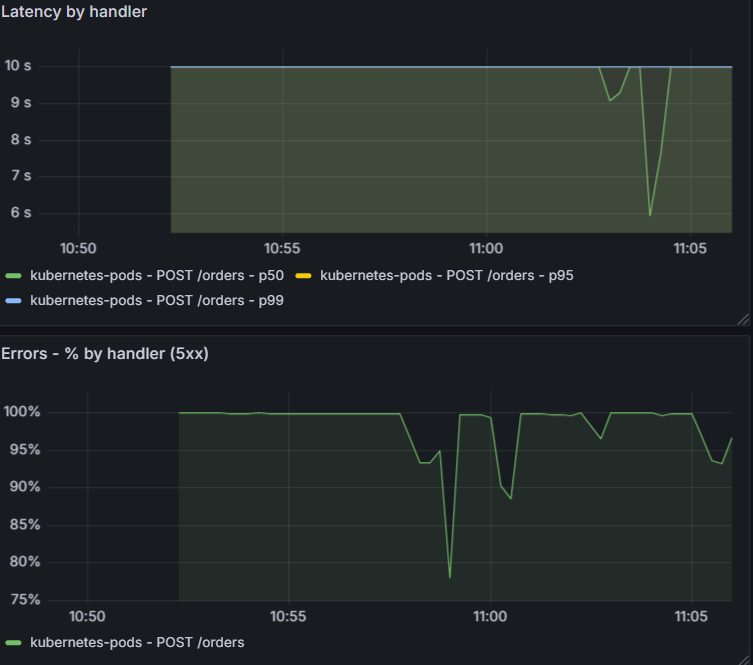
\includegraphics[width=0.8\textwidth]{resources/chapter-4/latensi-yugabyte-fail.png}
    \caption{Metrik Pemrosesan Pesanan (f3t2)}
    \label{fig:metrics-f3t2}
\end{figure}

Selama pengujian, terdapat beberapa kasus ketika salah satu \textit{node} YugabyteDB mati, sehingga menyebabkan kluster basis data mati dan tidak dapat menangani permintaan selama beberapa waktu. Kestabilan kluster ini juga merupakan hal yang menjadi permasalahan selama pengujian.

Setelah ditelusuri, laju pemrosesan kueri saat YugabyteDB mengalami kegagalan sebagaimana ditunjukkan pada gambar \ref{fig:metrics-f3t2} mengalami penurunan yang cukup tajam dibandingkan saat YugabyteDB berjalan cukup baik sebagiamana ditunjukkan pada gambar \ref{fig:metrics-f3t1}. Penyebab pasti hal ini belum dapat diidentifikasi hingga pengujian selesai dilaksanakan. Akan tetapi, dapat diasumsikan bahwa setelah melewati beban tertentu, YugabyteDB mulai kesulitan menangani beban yang diberikan, sehingga kegagalan mulai sering terjadi dan laju pemrosesan kueri menjadi lebih lambat.

Masalah lain yang berhasil diidentifikasi pada YugabyteDB ini adalah masalah manajemen koneksi. Setelah beberapa kali pengujian, tidak ditemukan kombinasi pengaturan koneksi yang memberikan kinerja yang baik, baik itu jumlah koneksi dari sisi klien ke PGCat atau pun jumlah koneksi dari PGCat ke TServer. \textit{Pooler} bawaan YugabyteDB, yaitu YSQL Connection Manager juga tidak memberikan perubahan kinerja. Selain itu, pengujian tanpa \textit{pooler} (menggunakan \textit{direct connection}) juga sudah dicoba dan tetap tidak memperoleh hasil yang baik.

Dari sisi \textit{throughput}, terdapat kasus ketika YugabyteDB memiliki hasil yang cukup baik sebagaimana ditunjukkan pada gambar berikut. Meskipun begitu, hasil ini tidak dapat direplikasi pada pengujian lain.

\begin{figure}[htbp]
    \centering
    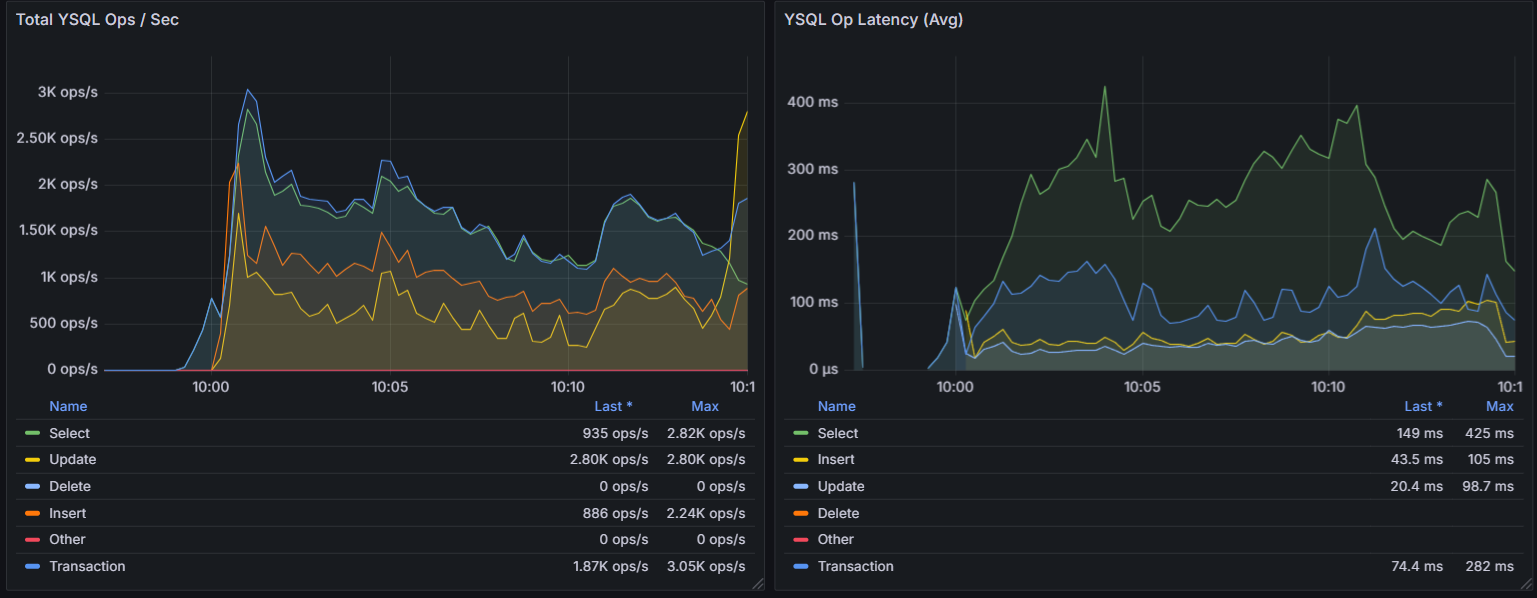
\includegraphics[width=1\textwidth]{resources/chapter-4/yugabyte-ops.png}
    \caption{\textit{Throughput} Kueri Pada YugabyteDB}
    \label{fig:yugabytedb-throughput}
\end{figure}

Singkat cerita, YugabyteDB kesulitan menangani beban koneksi yang ada pada pengujian dan memiliki masalah pada kestabilan kluster untuk dapat digunakan secara andal. Hal ini mungkin saja berubah apabila YugabyteDB diberi lebih banyak sumber daya atau lebih banyak \textit{node}.

\subsection{Pengoptimalan Kueri Baca}

\subsubsection{Kueri Ketersediaan Area}

Operasi baca ketersediaan area merupakan \textit{endpoint} yang cukup banyak dipanggil, terutama ketika ketersediaan tiket mulai menipis dan pengguna mencoba mengeksplorasi lebih banyak area. Pada pengujian f5t2, \textit{endpoint} ini memiliki puncak pemanggilan sebanyak 1700 rps. Sepanjang pengujian, latensi rata-rata operasi tersebut berkisar antara 2.5-4.5 milisekon. Hal ini menunjukkan bahwa pengoptimalan kueri ketersediaan area dengan menggunakan Redis merupakan pendekatan yang sangat efektif, terutama dalam meringankan beban pada basis data.

\pagebreak

\begin{figure}[htbp]
    \centering
    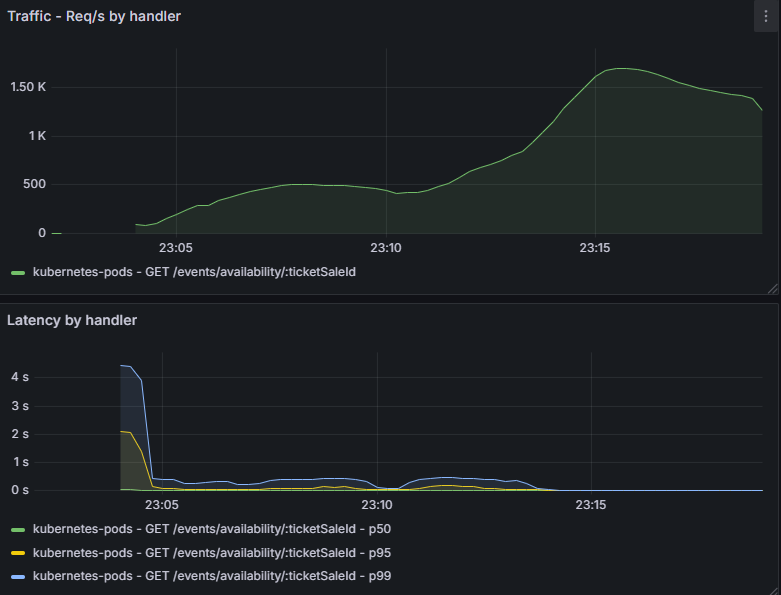
\includegraphics[width=0.8\textwidth]{resources/chapter-4/latency-area-availability.png}
    \caption{Metrik Baca Ketersediaan Area (f5t2)}
    \label{fig:latency-get-area}
\end{figure}

\subsubsection{Kueri Ketersediaan Kursi}

Operasi baca ketersediaan kursi tidak dipanggil sebanyak operasi sebelumnya. Hal ini karena tidak semua tiket merupakan tiket dengan nomor kursi dan pengguna tidak akan memanggil operasi ini apabila tidak menemukan area yang memenuhi kriterianya. Meskipun begitu, pengoptimalan kueri ini tidak berjalan dengan cukup baik sebagaimana ditunjukkan pada grafik berikut.

\begin{figure}[htbp]
    \centering
    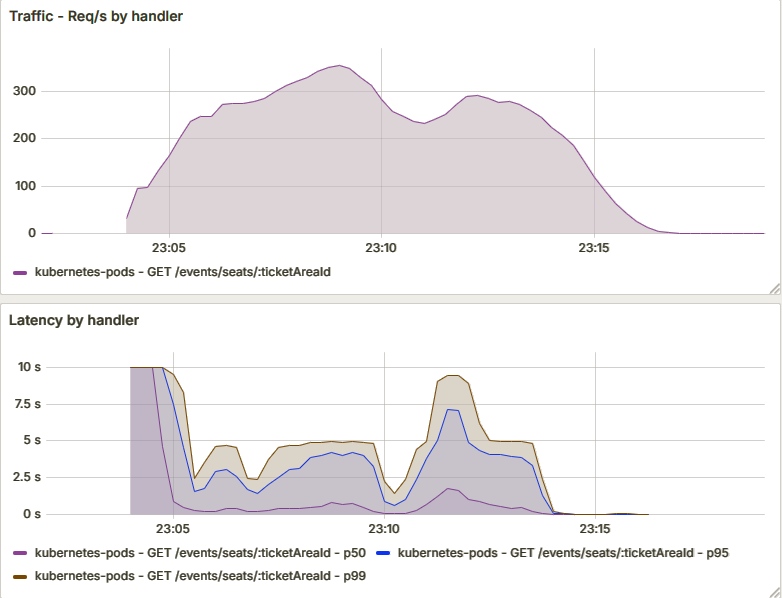
\includegraphics[width=0.8\textwidth]{resources/chapter-4/latency-seat-availability.png}
    \caption{Metrik Baca Ketersediaan Kursi (f5t2)}
    \label{fig:latency-get-seat}
\end{figure}

Rata-rata latensi (P50) memiliki nilai mulai dari 40 milisekon hingga 1.75 sekon (apabila mengesampingkan latensi di awal saat jumlah koneksi masih sedikit). Di sisi lain, latensi P95 cukup mengkhawatirkan dengan nilai mulai dari 1.6 sekon hingga 7 sekon. Hal ini menunjukkan bahwa penggunaan tembolok singkat (waktu hidup 150 milisekon) tidak begitu efektif. Hal ini terjadi karena beberapa hal berikut:

\begin{enumerate}
    \item Tembolok yang bersifat lokal pada level aplikasi.
    \item Sebaran pengguna yang membaca ID area yang berbeda-beda.
    \item Waktu hidup yang terlalu singkat.
\end{enumerate}

Kombinasi hal tersebut membuat \textit{cache hit} operasi ini sangat rendah sehingga tidak efektif. Selain itu, latensi ini menunjukkan bahwa operasi ini merupakan operasi yang cukup berat yang ditandai dengan latensi yang ada dan merupakan hal yang dapat menjadi fokus pengoptimalan di masa mendatang. Sebagaimana ditunjukkan pada pengoptimalan sebelumnya, pengoptimalan penggunaan Redis bisa menjadi alternatif yang dapat dieksplorasi lebih lanjut.

\subsection{Penggunaan Pengendalian Aliran}

Jelasin berapa banyak request yg ditolak (respons 409) -> respons 409 emang lebih banyak di flow control tapi kalau gitu harusnya jumlah yg ditolaknya sama gak sih? -> latensinya gede jadi pemrosesannya lama dan user ngira masih available padahal bakal enggak.

\begin{figure}[htbp]
    \centering
    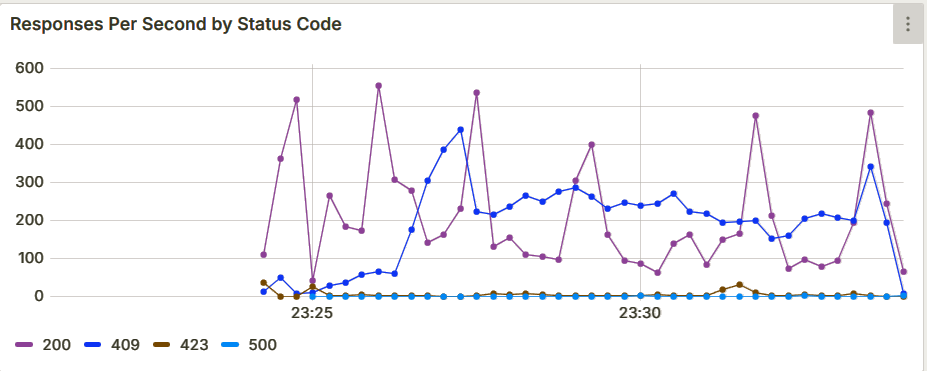
\includegraphics[width=0.6\textwidth]{resources/chapter-4/rps-fc-pg-stress-0.png}
    \caption{Laju Pemrosesan dengan Pengendalian Aliran}
    \label{fig:rps-fc-pg-stress-0}
\end{figure}

\begin{figure}[htbp]
    \centering
    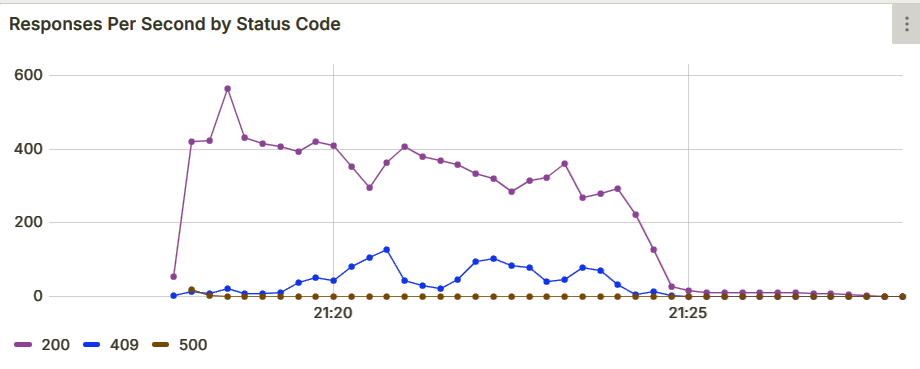
\includegraphics[width=0.6\textwidth]{resources/chapter-4/rps-nofc-pg-stress-0.png}
    \caption{Laju Pemrosesan tanpa Pengendalian Aliran}
    \label{fig:rps-nofc-pg-stress-0}
\end{figure}


ubah grafana dashboard agar bisa lihat latensi by response code -> bandingkan latensi pas 409 di flow control dan no flow control buat ngetes early dropper.

\begin{figure}[htbp]
    \centering
    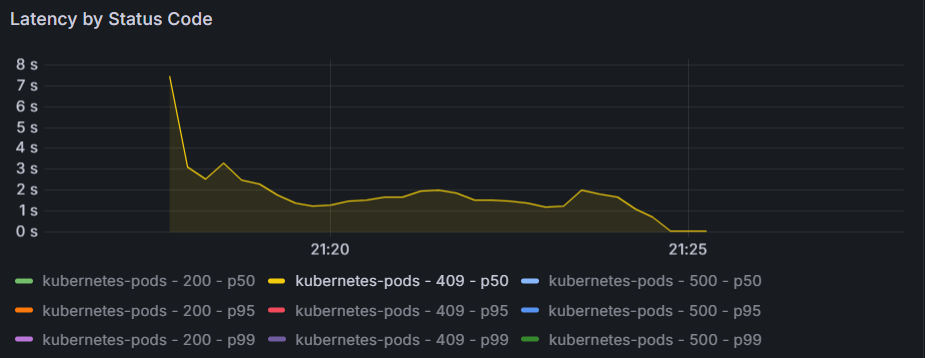
\includegraphics[width=0.6\textwidth]{resources/chapter-4/latency-by-code-nofc-pg-stress-0.png}
    \caption{Latensi Berdasarkan Status Kode tanpa Pengendalian Aliran}
    \label{fig:latency-by-code-nofc}
\end{figure}

\begin{figure}[htbp]
    \centering
    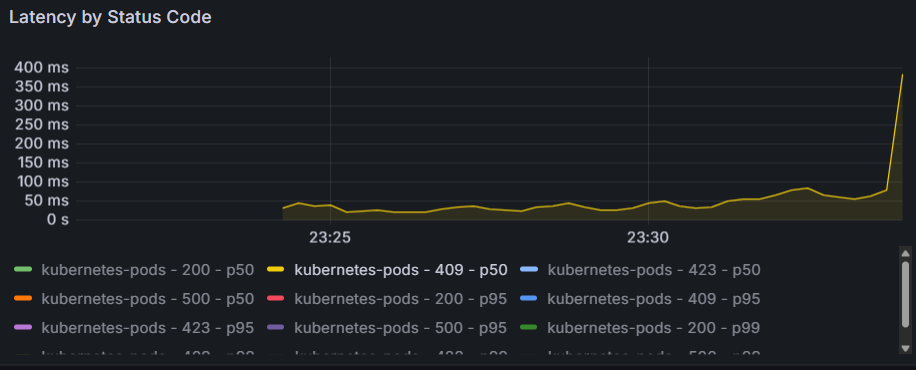
\includegraphics[width=0.6\textwidth]{resources/chapter-4/latency-by-code-fc-pg-stress-0.png}
    \caption{Latensi Berdasarkan Status Kode dengan Pengendalian Aliran}
    \label{fig:latency-by-code-fc}
\end{figure}

rabbitmq bikin latensi jadi terlalu tinggi -> gak feasible. ada side efek data kelamaan diupdate jg sebagaimana terjadi di atas.

latensi tinggi di sini karena overhead di rabbitmq dan kode yg butuh komunikasi dr backend ke worker terus worker kirim response.

\begin{figure}[htbp]
    \centering
    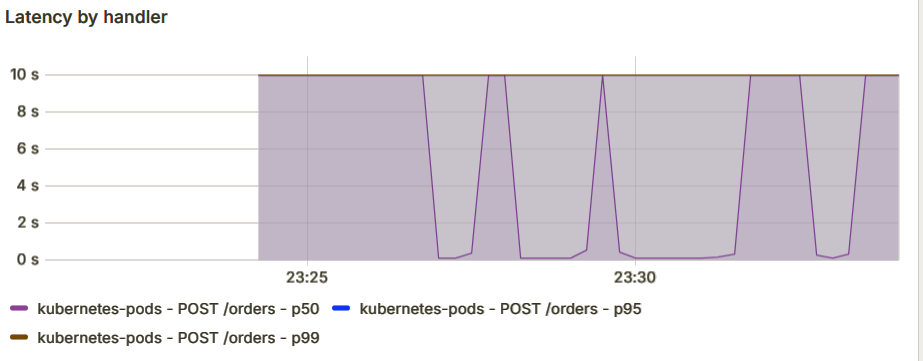
\includegraphics[width=0.6\textwidth]{resources/chapter-4/latency-fc-pg-stress-0.png}
    \caption{Latensi Pemrosesan dengan Pengendalian Aliran}
    \label{fig:latency-fc}
\end{figure}

\begin{figure}[htbp]
    \centering
    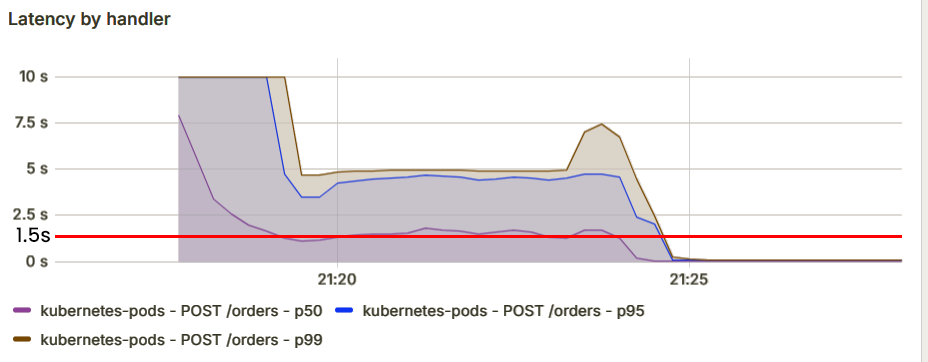
\includegraphics[width=0.6\textwidth]{resources/chapter-4/latency-nofc-pg-stress-0.png}
    \caption{Latensi Pemrosesan tanpa Pengendalian Aliran}
    \label{fig:latency-nofc}
\end{figure}

bandingkan latensi utk kueri related to processing tiket. kayaknya varian flow control lebih rendah (walau pun rabbitmq unintentionally make arrival order lebih lambat) tapi dengan jaga flow bisa terbukti lumayan cukup buat jaga latensi database.

verdict: (hopefully) early dropper konsepnya oke. buffer/ queue lebih baik per instance aja -> tapi harus mikirin gimana handle masalah idempotency (kalau retry user hrs dilempar ke instance yg sama).

todo integritas tiket di bawah: cek grafik yg kelihatan nol, aslinya nilainya gak nol itu.

\subsection{Integritas Tiket Selama Perebutan Tiket}

Pengoptimalan baca dengan menggunakan Redis memungkinkan terjadinya ketidakcocokan data antara basis data dengan hasil pengoptimalan. Di sisi lain, sistem juga harus memastikan bahwa tidak ada kursi yang terjual lebih dari satu kali. Oleh karena itu, terdapat tiga hal yang diperiksa untuk memastikan integritas sistem tiket:

\begin{enumerate}
    \item Selisih agregat ketersediaan antara basis data dengan Redis pada akhirnya harus nol untuk pengoptimalan operasi baca ketersediaan area.
    \item Selisih ketersediaan antara basis data dengan Redis pada akhirnya harus nol untuk pengoptimalan pengendalian aliran bagian penolakan permintaan lebih awal (hanya berlaku pada varian pengendalian aliran).
    \item Tidak ada kursi yang terjual lebih dari satu kali.
\end{enumerate}

Berikut adalah sampel hasil \textit{sanity check} selama pelaksanaan pengujian:

\begin{figure}[htbp]
    \centering
    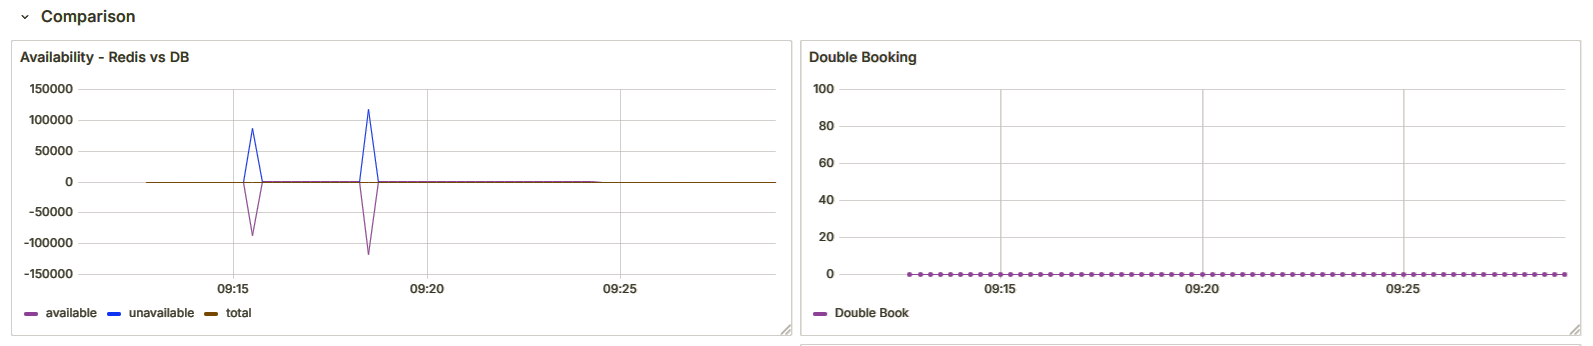
\includegraphics[width=1\textwidth]{resources/chapter-4/sanity-f2t3.png}
    \caption{Hasil \textit{Sanity Check} (f2t3)}
    \label{fig:sanity-f2t3}
\end{figure}

\begin{figure}[htbp]
    \centering
    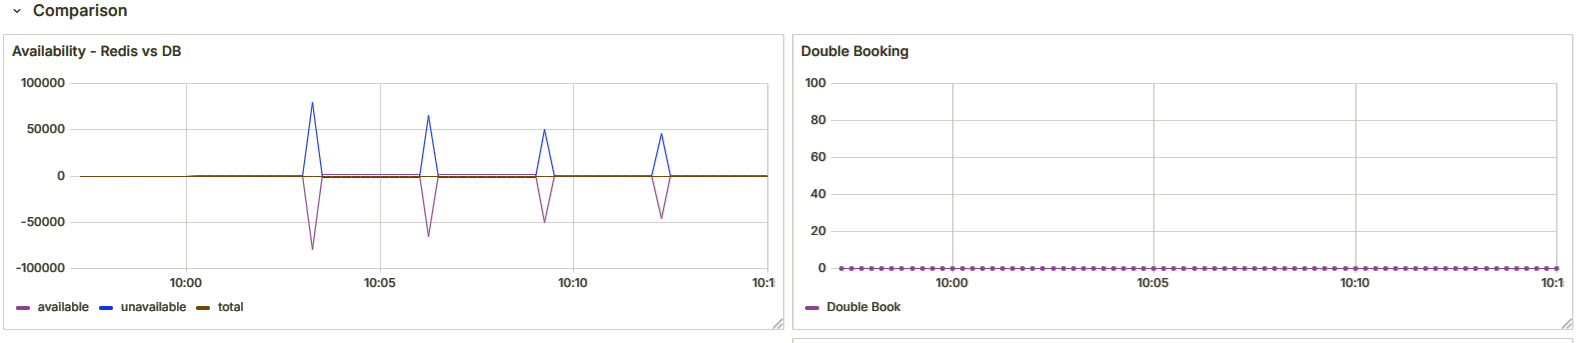
\includegraphics[width=1\textwidth]{resources/chapter-4/sanity-f3t1.png}
    \caption{Hasil \textit{Sanity Check} (f3t1)}
    \label{fig:sanity-f3t1}
\end{figure}

\begin{figure}[htbp]
    \centering
    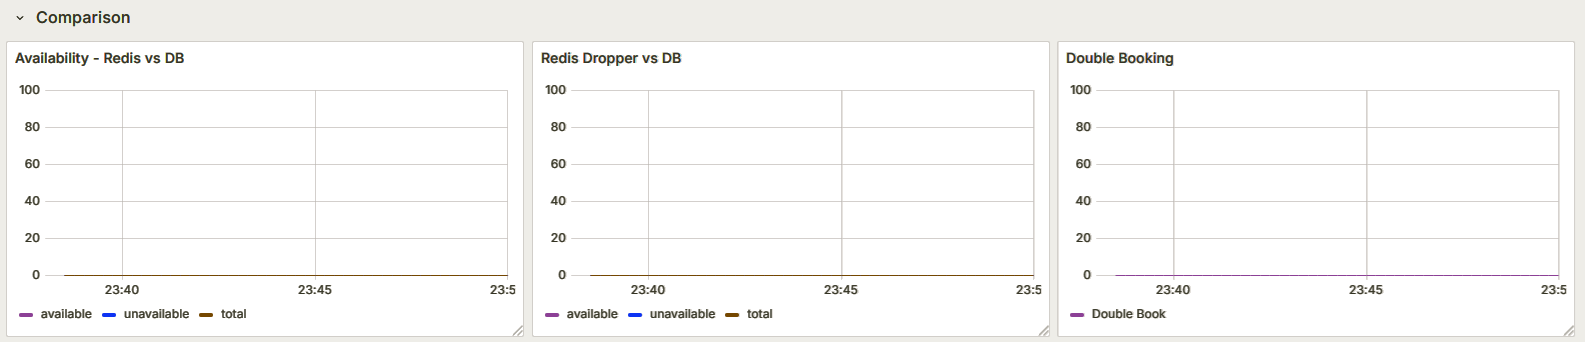
\includegraphics[width=1\textwidth]{resources/chapter-4/sanity-f5t4.png}
    \caption{Hasil \textit{Sanity Check} (f5t4)}
    \label{fig:sanity-f5t4}
\end{figure}

Berdasarkan sampel di atas, terdapat beberapa waktu terjadinya ketidaksesuaian data yang pada akhirnya konsisten. Setelah ditelusuri, hal tersebut terjadi karena masalah pada pengumpulan data yang mengalami kegagalan memperoleh data yang lengkap. Hal ini didukung dengan fakta bahwa selisih nilainya memang sangat ekstrem. Oleh karena itu, dapat disimpulkan bahwa implementasi yang ada sekarang telah menjamin kesesuaian data dan berhasil menjamin bahwa tidak ada kursi yang terjual lebih dari satu kali.
